% Template for PLoS
% Version 3.4 January 2017
\documentclass[10pt,letterpaper]{article}
\usepackage[top=0.85in,left=2.75in,footskip=0.75in]{geometry}

% amsmath and amssymb packages, useful for mathematical formulas and symbols
\usepackage{amsmath,amssymb}

% Use adjustwidth environment to exceed column width (see example table in text)
\usepackage{changepage}

% Use Unicode characters when possible
\usepackage[utf8x]{inputenc}

% textcomp package and marvosym package for additional characters
\usepackage{textcomp,marvosym}

% cite package, to clean up citations in the main text. Do not remove.
% \usepackage{cite}

% Use nameref to cite supporting information files (see Supporting Information section for more info)
\usepackage{nameref,hyperref}

% line numbers
\usepackage[right]{lineno}

% ligatures disabled
\usepackage{microtype}
\DisableLigatures[f]{encoding = *, family = * }

% color can be used to apply background shading to table cells only
\usepackage[table]{xcolor}

% array package and thick rules for tables
\usepackage{array}

% create "+" rule type for thick vertical lines
\newcolumntype{+}{!{\vrule width 2pt}}

% create \thickcline for thick horizontal lines of variable length
\newlength\savedwidth
\newcommand\thickcline[1]{%
  \noalign{\global\savedwidth\arrayrulewidth\global\arrayrulewidth 2pt}%
  \cline{#1}%
  \noalign{\vskip\arrayrulewidth}%
  \noalign{\global\arrayrulewidth\savedwidth}%
}

% \thickhline command for thick horizontal lines that span the table
\newcommand\thickhline{\noalign{\global\savedwidth\arrayrulewidth\global\arrayrulewidth 2pt}%
\hline
\noalign{\global\arrayrulewidth\savedwidth}}


% Remove comment for double spacing
%\usepackage{setspace} 
%\doublespacing

% Text layout
\raggedright
\setlength{\parindent}{0.5cm}
\textwidth 5.25in 
\textheight 8.75in

% Bold the 'Figure #' in the caption and separate it from the title/caption with a period
% Captions will be left justified
\usepackage[aboveskip=1pt,labelfont=bf,labelsep=period,justification=raggedright,singlelinecheck=off]{caption}
\renewcommand{\figurename}{Fig}

% Use the PLoS provided BiBTeX style
% \bibliographystyle{plos2015}

% Remove brackets from numbering in List of References
\makeatletter
\renewcommand{\@biblabel}[1]{\quad#1.}
\makeatother

% Leave date blank
\date{}

% Header and Footer with logo
\usepackage{lastpage,fancyhdr,graphicx}
\usepackage{epstopdf}
\pagestyle{myheadings}
\pagestyle{fancy}
\fancyhf{}
\setlength{\headheight}{27.023pt}
\lhead{\includegraphics[width=2.0in]{PLOS-submission.eps}}
\rfoot{\thepage/\pageref{LastPage}}
\renewcommand{\footrule}{\hrule height 2pt \vspace{2mm}}
\fancyheadoffset[L]{2.25in}
\fancyfootoffset[L]{2.25in}
\lfoot{\sf PLOS}

%% Include all macros below
\newcommand{\lorem}{{\bf LOREM}}
\newcommand{\ipsum}{{\bf IPSUM}}

\usepackage{color}
\usepackage{fancyvrb}
\newcommand{\VerbBar}{|}
\newcommand{\VERB}{\Verb[commandchars=\\\{\}]}
\DefineVerbatimEnvironment{Highlighting}{Verbatim}{commandchars=\\\{\}}
% Add ',fontsize=\small' for more characters per line
\usepackage{framed}
\definecolor{shadecolor}{RGB}{248,248,248}
\newenvironment{Shaded}{\begin{snugshade}}{\end{snugshade}}
\newcommand{\KeywordTok}[1]{\textcolor[rgb]{0.13,0.29,0.53}{\textbf{#1}}}
\newcommand{\DataTypeTok}[1]{\textcolor[rgb]{0.13,0.29,0.53}{#1}}
\newcommand{\DecValTok}[1]{\textcolor[rgb]{0.00,0.00,0.81}{#1}}
\newcommand{\BaseNTok}[1]{\textcolor[rgb]{0.00,0.00,0.81}{#1}}
\newcommand{\FloatTok}[1]{\textcolor[rgb]{0.00,0.00,0.81}{#1}}
\newcommand{\ConstantTok}[1]{\textcolor[rgb]{0.00,0.00,0.00}{#1}}
\newcommand{\CharTok}[1]{\textcolor[rgb]{0.31,0.60,0.02}{#1}}
\newcommand{\SpecialCharTok}[1]{\textcolor[rgb]{0.00,0.00,0.00}{#1}}
\newcommand{\StringTok}[1]{\textcolor[rgb]{0.31,0.60,0.02}{#1}}
\newcommand{\VerbatimStringTok}[1]{\textcolor[rgb]{0.31,0.60,0.02}{#1}}
\newcommand{\SpecialStringTok}[1]{\textcolor[rgb]{0.31,0.60,0.02}{#1}}
\newcommand{\ImportTok}[1]{#1}
\newcommand{\CommentTok}[1]{\textcolor[rgb]{0.56,0.35,0.01}{\textit{#1}}}
\newcommand{\DocumentationTok}[1]{\textcolor[rgb]{0.56,0.35,0.01}{\textbf{\textit{#1}}}}
\newcommand{\AnnotationTok}[1]{\textcolor[rgb]{0.56,0.35,0.01}{\textbf{\textit{#1}}}}
\newcommand{\CommentVarTok}[1]{\textcolor[rgb]{0.56,0.35,0.01}{\textbf{\textit{#1}}}}
\newcommand{\OtherTok}[1]{\textcolor[rgb]{0.56,0.35,0.01}{#1}}
\newcommand{\FunctionTok}[1]{\textcolor[rgb]{0.00,0.00,0.00}{#1}}
\newcommand{\VariableTok}[1]{\textcolor[rgb]{0.00,0.00,0.00}{#1}}
\newcommand{\ControlFlowTok}[1]{\textcolor[rgb]{0.13,0.29,0.53}{\textbf{#1}}}
\newcommand{\OperatorTok}[1]{\textcolor[rgb]{0.81,0.36,0.00}{\textbf{#1}}}
\newcommand{\BuiltInTok}[1]{#1}
\newcommand{\ExtensionTok}[1]{#1}
\newcommand{\PreprocessorTok}[1]{\textcolor[rgb]{0.56,0.35,0.01}{\textit{#1}}}
\newcommand{\AttributeTok}[1]{\textcolor[rgb]{0.77,0.63,0.00}{#1}}
\newcommand{\RegionMarkerTok}[1]{#1}
\newcommand{\InformationTok}[1]{\textcolor[rgb]{0.56,0.35,0.01}{\textbf{\textit{#1}}}}
\newcommand{\WarningTok}[1]{\textcolor[rgb]{0.56,0.35,0.01}{\textbf{\textit{#1}}}}
\newcommand{\AlertTok}[1]{\textcolor[rgb]{0.94,0.16,0.16}{#1}}
\newcommand{\ErrorTok}[1]{\textcolor[rgb]{0.64,0.00,0.00}{\textbf{#1}}}
\newcommand{\NormalTok}[1]{#1}




\usepackage{forarray}
\usepackage{xstring}
\newcommand{\getIndex}[2]{
  \ForEach{,}{\IfEq{#1}{\thislevelitem}{\number\thislevelcount\ExitForEach}{}}{#2}
}

\setcounter{secnumdepth}{0}

\newcommand{\getAff}[1]{
  \getIndex{#1}{Monash University,Genentech}
}

\providecommand{\tightlist}{%
  \setlength{\itemsep}{0pt}\setlength{\parskip}{0pt}}

\begin{document}
\vspace*{0.2in}

% Title must be 250 characters or less.
\begin{flushleft}
{\Large
\textbf\newline{plyranges: a grammar for transforming genomics data} % Please use "sentence case" for title and headings (capitalize only the first word in a title (or heading), the first word in a subtitle (or subheading), and any proper nouns).
}
\newline
\\
Stuart Lee\textsuperscript{\getAff{Monash University}},
Michael Lawrence\textsuperscript{\getAff{Genentech}},
Di Cook\textsuperscript{\getAff{Monash University}}\\
\bigskip
\textbf{\getAff{Monash University}}Department of Econometrics and Business Statistics, Clayton, Victoria,
Australia\\
\textbf{\getAff{Genentech}}Bioinformatics and Computational Biology, Genentech, Inc., South San
Francisco, California, United States of America\\
\bigskip
\end{flushleft}
% Please keep the abstract below 300 words
\section*{Abstract}
The Bioconductor project has created many useful data abstractions for
analysing high-throughput genomics experiments. However, there is a
cognitive load placed on a user in learning a data abstraction and
understanding its appropriate use. Throughout a standard workflow, a
user must navigate and know many of these abstractions to perform an
genomic analysis task, when a single data abstraction, a GRanges object
will suffice. The GRanges class naturally represent genomic intervals
and their associated measurements. By recognising that the GRanges class
follows `tidy' data principles we have created a grammar of genomic data
transformation. The grammar defines verbs for performing actions on and
between genomic interval data. It provides a principled way of
performing common genomic data analysis tasks through a coherent
interface to existing Bioconductor infrastructure, resulting in human
readable analysis workflows. We have implemented this grammar as an
Bioconductor/R package called plyranges.

% Please keep the Author Summary between 150 and 200 words
% Use first person. PLOS ONE authors please skip this step. 
% Author Summary not valid for PLOS ONE submissions.   

\linenumbers

% Use "Eq" instead of "Equation" for equation citations.
\section{Introduction}\label{introduction}

High-throughput genomics promises to unlock new disease therapies, and
strengthen our knowledge of basic biology. To deliver on those promises,
scientists must derive a stream of knowledge from a deluge of data.
Genomic data is challenging in both scale and complexity. Innovations in
sequencing technology often outstrip our capacity to process the output.
Beyond their common association with genomic coordinates, genomic data
are heterogeneous, consisting of raw sequence read alignments, genomic
feature annotations like genes and exons, and summaries like coverage
vectors, ChIP-seq peak calls, variant calls, and per-feature read
counts. Genomic scientists need software tools to wrangle the different
types of data, process the data at scale, test hypotheses, and generate
new ones, all while focusing on the biology, not the computation. For
the tool developer, the challenge is to define ways to model and operate
on the data that align with the mental model of scientists, and to
provide an implementation that scales with their ambition.

Several domain specific languages (DSLs) enable scientists to process
and reason about heterogeneous genomics data heterogeneous genomics data
by expressing common operations, such as range manipulation and
overlap-based joins, using the vocabulary of genomics. Their
implementations either delegate computations to a database, or operate
over collections of files in standard formats like BED.An example of the
former is the Genome Query Language (GQL) and its distributed
implementation GenAp which use an SQL-like syntax for fast retrieval of
information of unprocessed sequencing data {[}1{]}; {[}2{]}. Similarly,
the Genometric Query Language (GMQL) implements a relational algebra for
combining genomic datasets {[}3{]}. The command line application
BEDtools develops an extensive algebra for performing arithmetic between
two or more sets of genomic regions {[}4{]}. All of the aforementioned
DSLs are designed to be evaluated either at the command line or embedded
in scripts for batch processing. They exist in sparse ecosystem, mostly
consisting of UNIX and database tools that lack biological semantics and
operate at the level of files and database tables.

The Bioconductor/R packages \texttt{IRanges} and \texttt{GenomicRanges}
{[}5--7{]} define a DSL for analysing genomics data with R, an
interactive data analysis environment that encourages reproducibility
and provides high-level abstractions for manipulating, modelling and
plotting data, through state of the art methods in statistical
computing. The packages define object-oriented (OO) abstractions for
representing genomic data and enable interoperability by allowing users
and developers to use these abstractions in their own code and packages.
Other genomic DSLs that are embedded in programming languages include
pybedtools and valr {[}8,9{]}, however these packages lack the
interoperability provided by in the aforementioned Bioconductor packages
and are not easily extended.

The Bioconductor infrastructure models the genomic data and operations
from the perspective of the power user, one who understands and wants to
take advantage of the subtle differences in data types. This design has
enabled the development of sophisticated tools, as evidenced by the
hundreds of packages depending the framework. Unfortunately, the myriad
of data structures have overlapping purposes and important but obscure
differences in behaviour that often confuse the typical end user.

Recently, there has been a concerted, community effort to standardize R
data structures and workflows around the notion of tidy data {[}10{]}. A
tidy dataset is defined to be to a tabular data structure that has
observations as rows and columns as variables, and each tidy dataset
represents measurements from a single observational unit. The tidy data
pattern is useful because it allows us to see how the data relates to
the design of an experiment and the variables measured. The
\texttt{dplyr} package {[}11{]} defines an API that maps notions from
the general relational algebra to operations on tidy data. It expresses
each operation as a cohesive, endomorphic verb. Taken together these
features enable a user to write human readable analysis workflows.

We have created a genomic DSL called \texttt{plyranges} that
reformulates notions from existing genomic algebras and embeds them in R
as a genomic extension of \texttt{dplyr}. By analogy, \texttt{plyranges}
is to the genomic algebra, as \texttt{dplyr} is to the relational
algebra. The \texttt{plyranges} Bioconductor package implements the
language on top of a key subset of Bioconductor data structures and thus
fully integrates with the Bioconductor framework, gaining access to its
scalable data representations and sophisticated statistical methods.

\section{Design and Implementation}\label{design-and-implementation}

The \texttt{plyranges} DSL is built on the most general Bioconductor
data structure, GRanges, which is capable of representing all types of
genomic data at a semantic level that roughly matches the intuition of
most users. A GRanges is essentially a table, with columns for the
chromosome, start and end coordinates, and the strand, along with an
arbitrary set of additional columns, consisting of measurements or
metadata specific to the data type or experiment. For example a GRanges
can be used to represent a gene with its chromosomal coordinates, and
along with its exon identifiers; or a GRanges can represent an RNA-seq
experiment as a set of genes with a corresponding count column.

By definition the GRanges follow the tidy data pattern: it is a
rectangular table corresponding to a single biological context. Each row
contains a single observation and each column is a variable about that
observation. Hence, we have designed the \texttt{plyranges} DSL to
extend the grammar and design principles of \texttt{dplyr}: cohesion,
consistency, endomorphism, and fluency. All of these principles are
defined and discussed below in the context of the GRanges class. Where
applicable we contrast our design to the existing Bioconductor
infrastructure.

\subsection{Cohesion}\label{cohesion}

A function is cohesive if it performs a singular task and does not
produce any side-effects. In the \texttt{plyranges} DSL our algebra for
performing genomic arithmetic is a key example of cohesion. We define
anchoring operators that decorate a GRanges object with an `anchor' and
modify the semantics of performing genomic arithmetic. The anchoring
operators amount to fixing a GRanges object by its start, center, or end
coordinates (or fixing these coordinates by strand). This enables any
arithmetic function that performs a coordinate transformation to remain
cohesive: that is they always perform the same operation regardless of
whether a GRanges object is anchored or not. The only difference is the
result of performing the arithmetic changes when contextual information
is added to the GRanges object.

Another example of our algebra altering object semantics, while
maintaining cohesion is through the `group\_by' operator. Like
anchoring, this operator decorates a GRanges object with a column name
(or names) that defines a partitioning of the GRanges by the unique
values in the column(s). Functions defined in the \texttt{plyranges} DSL
that perform restriction, aggregation, or column modification still
perform those singular tasks, however grouping changes how those tasks
are performed.

Our algebra recasts the actions of finding overlaps or nearest
neighbours between two genomic regions as a relational join operator.
The join operator acts on two GRanges object, a query and a subject. The
join operator is relational in the sense that metadata from the query
and subject ranges is retained in the joined range. The commonality
between all join operators in the \texttt{plyranges} DSL is to use the
index of where in the query range the subject range `hits' the query
range as a primary key (figure \emph{need to make figure}). The notion
of `hits' and hence the resulting key is determined by the type of join
(preceding, nearest, follows overlaps).

We extend this idea by introducing three types of overlap joins: inner,
intersect and left. The inner join considers a hit to be any overlap
between subject and query and expands the query range to have length
equal to the number of hits. The intersect join uses the same definition
of a hit as the inner join but returns a range where the start and end
coordinates are the intersect of coordinates in the subject that hit the
query. Finally, the overlap left join is akin to left outer join in
Cobb's relational algebra: it performs an overlap inner join but also
returns all query ranges that are not hit by the subject.

The behaviour of a join operator can be further altered with additional
suffixes by restricting or expanding how a subject `hits' a query. For
example, for overlap joins we can use suffixes to encapsulate Allan's
Interval Algebra: to consider subject `hits' that are entirely `within'
a query range, the `within' prefix is used. We also use the `directed'
suffix to explicitly include notions of strandedness in our algebra.

more comparison to Bioconductor API here? table of join ops?

\subsection{Consistency}\label{consistency}

A core design principle of the \texttt{plyranges} DSL is interface
consistency: a user should not be surprised by the input or output of
\texttt{plyranges} code. A key example of consistency is how
\texttt{plyranges} handles strand information. Every function that
computes with strand information indicates its intentions by including
suffixes such as `directed', `upstream' or `downstream' in its name,
otherwise strand is ignored. This strongly differs from the Bioconductor
packages, which produces surprising output by assuming the user is
always interested in using strand in the majority of circumstances
(unless a user is computing coverage or finding flanking ranges).

Our use of suffixes in function names, also highlights are core tenet of
the \texttt{plyranges} design: avoid complex generic functions with many
arguments and instead use cohesive functions with a minimal number of
arguments. As an example, we have written a consistent framework for
reading and writing files from and to common genomic data formats as
GRanges, using the \texttt{rtracklayer} package as a back-end {[}12{]}.
We have replaced that packages generic functions for importing files
with a family of reader functions that all take the exact same
arguments.

\subsection{Endomorphism}\label{endomorphism}

Most function calls in \texttt{plyranges} are endomorphisms: when the
input is GRanges object the output will also be a GRanges object. The
use of endomorphism in the \texttt{plyranges} DSL enables a user to
predict the structure of the output of their computations and does not
require them to learn any additional classes beyond GRanges and
DataFrames.

This design pattern strongly deviates from the design of the OO
interface in \texttt{GenomicRanges}, where many methods return a new
class that is unfamiliar to the user upon return. These low-level
classes enable efficient computing at the cost of complexity and are
abstracted away in \texttt{plyranges} interface.

\subsection{Fluency}\label{fluency}

As a consequence of the design principles defined above every function
in \texttt{plyranges} performs a single action on GRanges objects. The
\texttt{plyranges} DSL implements the core verbs from the \texttt{dplyr}
package and implements a genomic relational algebra for transforming
GRanges objects (table x, y). Each verb preserves the semantics of
GRanges object and works with derivatives of the GRanges class. Both of
these aspects reduce the cognitive load on a new user since most
manipulations can be performed with a vocabulary of several verbs,
rather than having to memorise function names that are nouns.

This approach strongly contrasts the \texttt{GenomicRanges/IRanges} OO
interface, which emphasises the use of setter and getter methods. In
that interface, core components and metadata are updated via replacement
methods (requiring knowledge of the class components), while our
interface requires only a single call to \texttt{mutate()} to perform
the modification.

Workflows can be composed by chaining verbs together into `sentences'
via the forward pipe operator,\texttt{\%\textgreater{}\%} (exported from
the R package \texttt{magrittr} {[}13{]}), which can be read as the word
`then'. Overall, this allows users to write human readable code because
workflows describe what the code is doing rather than how its doing it.

\subsection{Limitations}\label{limitations}

A caveat to constructing a compatible interface with \texttt{dplyr} is
that \texttt{plyranges} makes extensive use of non-standard evaluation
in R (achieved via the \texttt{rlang} package {[}14{]}). Simply, this
means that computations are performed and evaluated in the context of
the GRanges objects, which emphasises the interactive nature of the
interface. This has the disadvantage that programming with
\texttt{plyranges} becomes more difficult because a user needs to know
about non-standard evaluation and user defined functions can be
difficult to debug.

\section{Results}\label{results}

Here we provide examples on how to use the \texttt{plyranges} DSL to
construct genomic data workflows.

\subsection{Peak Finding}\label{peak-finding}

We use the Bioconductor package \emph{AnnotationHub} {[}15{]} to search
for BigWig files from ChIP-Seq experiments from the Human Epigenome
Roadmap project {[}16{]}. We choose to focus on assays for primary T
CD8+ memory cells from peripheral blood. We can then read the BigWig
file corresponding to the H3 lysine 27 trimethylation (H3K27Me3)
methylation mark over chromosome 10.

First, we gather the BigWig file and extract its annotation information
and filter it to chromosome 10.

\begin{Shaded}
\begin{Highlighting}[]
\KeywordTok{library}\NormalTok{(plyranges)}
\NormalTok{chr10_ranges <-}\StringTok{ }\NormalTok{bw_file }\OperatorTok\StringTok{ }
\StringTok{  }\KeywordTok{get_genome_info}\NormalTok{() }\OperatorTok
\StringTok{  }\KeywordTok{filter}\NormalTok{(seqnames }\OperatorTok{==}\StringTok{ "chr10"}\NormalTok{)}
\end{Highlighting}
\end{Shaded}

Then we read the BigWig file only extracting scores if they overlap
chromosome 10. The annotation information from the file is automatically
included (in this case the hg19 genome build).

\begin{Shaded}
\begin{Highlighting}[]
\NormalTok{chr10_scores <-}\StringTok{ }\NormalTok{bw_file }\OperatorTok
\StringTok{  }\KeywordTok{read_bigwig}\NormalTok{(}\DataTypeTok{overlap_ranges =}\NormalTok{ chr10_ranges) }\OperatorTok
\StringTok{  }\KeywordTok{set_genome_info}\NormalTok{(}\DataTypeTok{genome =} \StringTok{"hg19"}\NormalTok{)}
\NormalTok{chr10_scores}
\end{Highlighting}
\end{Shaded}

\begin{verbatim}
#> GRanges object with 5789841 ranges and 1 metadata column:
#>             seqnames                 ranges strand |              score
#>                <Rle>              <IRanges>  <Rle> |          <numeric>
#>         [1]    chr10         [    1, 60602]      * | 0.0422799997031689
#>         [2]    chr10         [60603, 60781]      * |  0.163240000605583
#>         [3]    chr10         [60782, 60816]      * |  0.372139990329742
#>         [4]    chr10         [60817, 60995]      * |  0.163240000605583
#>         [5]    chr10         [60996, 61625]      * | 0.0422799997031689
#>         ...      ...                    ...    ... .                ...
#>   [5789837]    chr10 [135524723, 135524734]      * |  0.144319996237755
#>   [5789838]    chr10 [135524735, 135524775]      * |  0.250230014324188
#>   [5789839]    chr10 [135524776, 135524784]      * |  0.427789986133575
#>   [5789840]    chr10 [135524785, 135524806]      * |  0.730019986629486
#>   [5789841]    chr10 [135524807, 135524837]      * |   1.03103005886078
#>   -------
#>   seqinfo: 25 sequences from hg19 genome
\end{verbatim}

The \texttt{reduce\_ranges()} operation is used to find coverage peaks
across chromosome 10. We can manually set a threshold to restrict
genomic regions to have a coverage score of greater than 8, and then
merge nearby regions. The maximum coverage is computed over all the
coverage scores in the regions that were reduced.

\begin{Shaded}
\begin{Highlighting}[]
\NormalTok{all_peaks <-}\StringTok{ }\NormalTok{chr10_scores }\OperatorTok\StringTok{ }
\StringTok{  }\KeywordTok{filter}\NormalTok{(score }\OperatorTok{>}\StringTok{ }\DecValTok{8}\NormalTok{) }\OperatorTok\StringTok{ }
\StringTok{  }\KeywordTok{reduce_ranges}\NormalTok{(}\DataTypeTok{score =} \KeywordTok{max}\NormalTok{(score))}
\end{Highlighting}
\end{Shaded}

Returning to the GRanges object containing normalised coverage scores
for the methylation data, we can filter to find the coordinates of the
peak containing the maximum coverage score. We can then find a 5000 nt
region centered around the maximum position by anchoring and modifying
the the width.

\begin{Shaded}
\begin{Highlighting}[]
\NormalTok{chr10_max_score_region <-}\StringTok{ }\NormalTok{chr10_scores }\OperatorTok
\StringTok{  }\KeywordTok{filter}\NormalTok{(score }\OperatorTok{==}\StringTok{ }\KeywordTok{max}\NormalTok{(score)) }\OperatorTok\StringTok{ }
\StringTok{  }\KeywordTok{anchor_center}\NormalTok{() }\OperatorTok
\StringTok{  }\KeywordTok{set_width}\NormalTok{(}\DecValTok{5000}\NormalTok{)}
\end{Highlighting}
\end{Shaded}

Finally, the overlap inner join is used to restrict the chromosome 10
normalised coverage scores that are within the 5000nt region that
contain the max peak on chromosome 10 (visualised in figure
\ref{fig:peak-viz}).

\begin{Shaded}
\begin{Highlighting}[]
\NormalTok{peak_region <-}\StringTok{ }\NormalTok{chr10_scores }\OperatorTok
\StringTok{  }\KeywordTok{join_overlap_inner}\NormalTok{(chr10_max_score_region)}
\end{Highlighting}
\end{Shaded}

\begin{figure}

{\centering 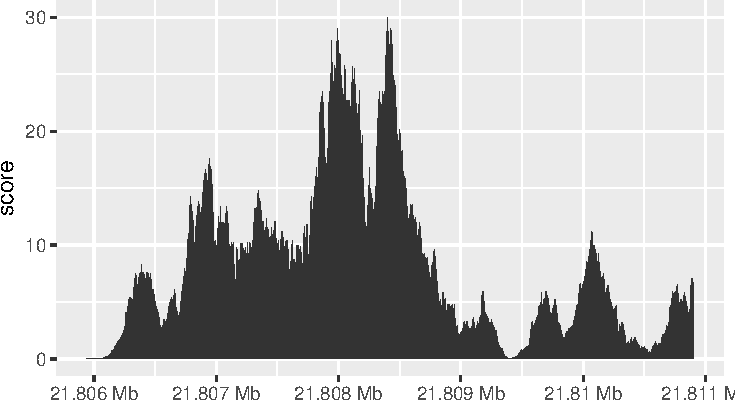
\includegraphics{paper_files/figure-latex/peak-viz-1} 

}

\caption{Visualisation of normalised coverage scores accross a 5000nt region of chromosome 10 from H3K27Me3 ChIP-Seq assay from the Human Epigenome Roadmap project.}\label{fig:peak-viz}
\end{figure}

\subsection{Computing Windowed
Statistics}\label{computing-windowed-statistics}

(example of group\_by\_overlaps + summarise)

\subsection{Transition Transversion
Ratio}\label{transition-transversion-ratio}

(example of group\_by + mutate + summarise and working on an object that
inherits from GRanges)

\section{Availablilty and Future
Work}\label{availablilty-and-future-work}

The \emph{plyranges} package is available on the Bioconductor project
website \url{https://bioconductor.org} or can be accessed via Github
\url{https://github.com/sa-lee/plyranges}. We aim to continue developing
the \texttt{plyranges} package and extend it for use with more complex
data structures such as the \emph{SummarizedExperiment} class, which can
be used for analysing transcriptomic and variant data. As the
\texttt{plyranges} interface encourages tidy data practices it
integrates well with the principles of the grammar of graphics, we aim
to use it to prepare data for the visualisation of multimodal biological
datasets.

\section*{References}\label{references}
\addcontentsline{toc}{section}{References}

\hypertarget{refs}{}
\hypertarget{ref-Kozanitis2014-va}{}
1. Kozanitis C, Heiberg A, Varghese G, Bafna V. Using genome query
language to uncover genetic variation. Bioinformatics. 2014;30: 1--8.
doi:\href{https://doi.org/10.1093/bioinformatics/btt250}{10.1093/bioinformatics/btt250}

\hypertarget{ref-Kozanitis2016-bm}{}
2. Kozanitis C, Patterson DA. GenAp: A distributed SQL interface for
genomic data. BMC Bioinformatics. 2016;17: 63.
doi:\href{https://doi.org/10.1186/s12859-016-0904-1}{10.1186/s12859-016-0904-1}

\hypertarget{ref-Kaitoua2017-pw}{}
3. Kaitoua A, Pinoli P, Bertoni M, Ceri S. Framework for supporting
genomic operations. IEEE Trans Comput. 2017;66: 443--457.
doi:\href{https://doi.org/10.1109/TC.2016.2603980}{10.1109/TC.2016.2603980}

\hypertarget{ref-Quinlan2010-gc}{}
4. Quinlan AR, Hall IM. BEDTools: A flexible suite of utilities for
comparing genomic features. Bioinformatics. 2010;26: 841--842.
doi:\href{https://doi.org/10.1093/bioinformatics/btq033}{10.1093/bioinformatics/btq033}

\hypertarget{ref-r-core}{}
5. R Core Team. R: A language and environment for statistical computing
{[}Internet{]}. Vienna, Austria: R Foundation for Statistical Computing;
2018. Available: \url{https://www.R-project.org/}

\hypertarget{ref-Lawrence2013-wg}{}
6. Lawrence M, Huber W, Pagès H, Aboyoun P, Carlson M, Gentleman R, et
al. Software for computing and annotating genomic ranges. PLoS Comput
Biol. 2013;9.
doi:\href{https://doi.org/10.1371/journal.pcbi.1003118}{10.1371/journal.pcbi.1003118}

\hypertarget{ref-Huber2015-ei}{}
7. Huber W, Carey VJ, Gentleman R, Anders S, Carlson M, Carvalho BS, et
al. Orchestrating high-throughput genomic analysis with bioconductor.
Nat Methods. Springer Nature; 2015;12: 115--121.
doi:\href{https://doi.org/10.1038/nmeth.3252}{10.1038/nmeth.3252}

\hypertarget{ref-Dale2011-js}{}
8. Dale RK, Pedersen BS, Quinlan AR. Pybedtools: A flexible python
library for manipulating genomic datasets and annotations.
Bioinformatics. 2011;27: 3423--3424.
doi:\href{https://doi.org/10.1093/bioinformatics/btr539}{10.1093/bioinformatics/btr539}

\hypertarget{ref-Kent2017}{}
9. Riemondy KA, Sheridan RM, Gillen A, Yu Y, Bennett CG, Hesselberth JR.
Valr: Reproducible genome interval arithmetic in r. F1000Research. 2017;
doi:\href{https://doi.org/10.12688/f1000research.11997.1}{10.12688/f1000research.11997.1}

\hypertarget{ref-Wickham2014-jc}{}
10. Wickham H. Tidy data. Journal of Statistical Software, Articles.
2014;59: 1--23.
doi:\href{https://doi.org/10.18637/jss.v059.i10}{10.18637/jss.v059.i10}

\hypertarget{ref-Wickham2017-dplyr}{}
11. Wickham H, Francois R, Henry L, Müller K. Dplyr: A grammar of data
manipulation {[}Internet{]}. 2017. Available:
\url{https://CRAN.R-project.org/package=dplyr}

\hypertarget{ref-Lawrence2009-nt}{}
12. Lawrence M, Gentleman R, Carey V. Rtracklayer: An R package for
interfacing with genome browsers. Bioinformatics. 2009;25: 1841--1842.
doi:\href{https://doi.org/10.1093/bioinformatics/btp328}{10.1093/bioinformatics/btp328}

\hypertarget{ref-R-magrittr}{}
13. Bache SM, Wickham H. Magrittr: A forward-pipe operator for r
{[}Internet{]}. 2014. Available:
\url{https://CRAN.R-project.org/package=magrittr}

\hypertarget{ref-R-rlang}{}
14. Henry L, Wickham H. Rlang: Functions for base types and core r and
'tidyverse' features {[}Internet{]}. 2017. Available:
\url{http://rlang.tidyverse.org}

\hypertarget{ref-R-ahub}{}
15. Morgan M. AnnotationHub: Client to access annotationhub resources.
2017.

\hypertarget{ref-Roadmap_Epigenomics_Consortium2015-pr}{}
16. Roadmap Epigenomics Consortium, Kundaje A, Meuleman W, Ernst J,
Bilenky M, Yen A, et al. Integrative analysis of 111 reference human
epigenomes. Nature. 2015;518: 317--330.
doi:\href{https://doi.org/10.1038/nature14248}{10.1038/nature14248}

\nolinenumbers


\end{document}

